\begin{frame}{Highlevel Front-End Development}

    In general, Front-End developement  cover merely these two things.

    \begin{enumerate}
        \item  $ F_1(S) = U $ : Translate raw data to fancy UI.
        \item  $ F_2(S_{old},A)=S_{new} $ : Map user action to state transform.
    \end{enumerate}

    \begin{itemize}
        \pause
        \item \textbf{S}: Page State 
        \pause
        \item \textbf{U}: User Interface (e.g. Html and CSS)
        \pause
        \item \textbf{A}: User Actions. (e.g. click a button)
        \pause
        \item \textbf{$F_x$}: The code you write.
    \end{itemize}

    \pause


    

    
\end{frame}

\begin{frame}

    The most difficult part of fe-dev is how to \textbf{manage} the \textbf{state}

    There are lots of tries to solve  this problem

    \begin{itemize}
        \item MVC Framework: Django , Rails, JSP...
        \item MVVM Framework: Vue, WPF
    \end{itemize}

    \begin{columns}
        \begin{column}{.2\textwidth}
    \begin{figure}
        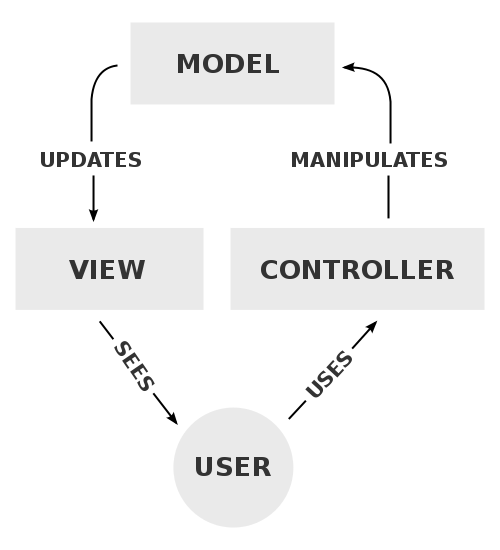
\includegraphics[width=\textwidth]{assets/MVC.png}
        \caption{MVC}
    \end{figure}
        \end{column}
    \end{columns}
\end{frame}
\begin{frame}
    \begin{figure}
        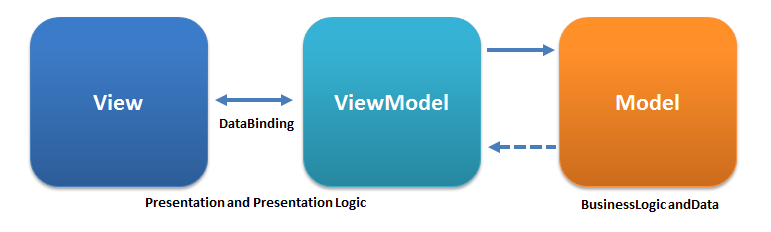
\includegraphics[width=.8\textwidth]{assets/MVVM.png}
        \caption{MVVM Diagram }
    \end{figure}

\end{frame}

\begin{frame}

    The most difficult part of fe-dev is how to \textbf{manage} the \textbf{state}

    There are lots of tries to solve  this problem

    \begin{itemize}
        \item MVC Framework: Django , Rails, JSP...
        \item MVVM Framework: Vue, WPF
    \end{itemize}

\end{frame}